\documentclass{beamer}
\usepackage[utf8]{inputenc}
\usepackage[autostyle]{csquotes}
\usepackage{fancybox}
\usepackage{graphicx}
%\usepackage{subcaption}
\usepackage{tabulary}
\usepackage{tabularx}
\usepackage[export]{adjustbox}
%\usepackage[style=numeric]{biblatex}
%\addbibresource{library.bib}
 
 
\title{Yubikey Wat is dat? Wat kann dat?}
\author{judge}
\date{}

\usetheme{metropolis}
\usecolortheme{default}

\begin{document}
 
\frame{\titlepage}

%\section{One Key to rule them all}
\begin{frame}
\frametitle{One Key to rule them all}
	\begin{figure}[h]
		\center
		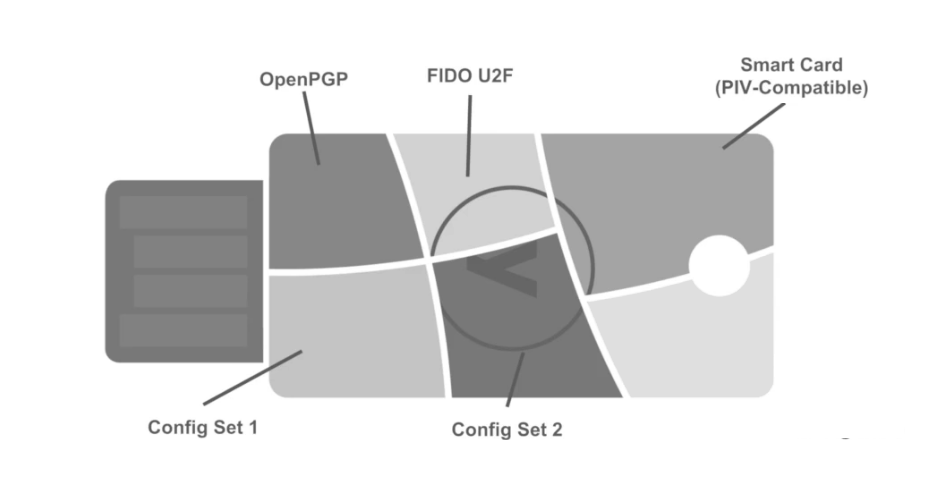
\includegraphics[width=0.7\textwidth]{images/functionality.png}
	\end{figure}
	\begin{columns}
		\column{0.33\textwidth}
			\pause
			\textbf{Config Slots}
			\begin{itemize}
				\item<3->{Synchrone Verschlüsselung}
				\item<3->{Challenge Response}
				\item<3->{Yubico OTP}
			\end{itemize}
		\column{0.33\textwidth}
			\textbf{PGP Smartcard}
			\begin{itemize}
				\item<4->{Asynchrone Verschlüsselung}
				\item<4->{Encryption}
				\item<4->{Signing}
				\item<4->{Authentication}
			\end{itemize}
		\column{0.33\textwidth}
			\textbf{PIV Smartcard}
			\begin{itemize}
				\item<5->{Asynchrone Verschlüsselung}
				\item<5->{4 Slots usable for multiple purposes}
			\end{itemize}
	\end{columns}
\end{frame}

\begin{frame}
\frametitle{Second Factor}
\end{frame}

\begin{frame}
\frametitle{Rechner login}
\end{frame}

\begin{frame}
\frametitle{SSH Authentication}
\end{frame}

\end{document}

%	\begin{columns}
%		\column{0.45\textwidth}
%			\begin{itemize}
%				\item<1->{proprietary bluetooth protocol}
%				\item<1->{detects 5 predefined gestures}
%				\item<2->{access to raw IMU and EMG data}
%			\end{itemize}
%		\column{0.55\textwidth}
%			\begin{figure}[h]
%				\center
%				\includegraphics[width=1\textwidth]{images/myo_armband.jpg}
%				\caption{MYO stock photo\cite{myopic}}
%			\end{figure}
%	\end{columns}
